%-Document Type------------------------------------------------------------------------------
\documentclass[12pt,a4paper]{report}
%--------------------------------------------------------------------------------------------

%Packages------------------------------------------------------------------------------------
\usepackage[colorlinks=true,linkcolor=blue]{hyperref} %Using this package will automatically turn references into links.
\usepackage{graphicx}
\usepackage{listings} % Required for insertion of code
\usepackage[linesnumbered]{algorithm2e}
\usepackage{tikz}
\usepackage{verbatim}
\usepackage{subcaption}
\usepackage{hyperref}
\usetikzlibrary{trees}
%---------------------------------------------------------------------------------------------

%Preamble-------------------------------------------------------------------------------------

%End Preamble---------------------------------------------------------------------------------

%Document----------------------------------------------------------------------------------------
\begin{document}
\parindent0pt

%Cover Page---------------------------------------------------------------------------------------
\title{COMS3: Advanced Analysis of Algorithms Assignment}
\author{Tau Merand 908096 \and Vincent Varkevisser 705668}
\maketitle
%Cover Page End-----------------------------------------------------------------------------------
\section*{Introduction}
The game of peg solitaire is a one player game played on a 33 holed cross shaped board that involves jumping pegs over other pegs, in a manner similar to checkers. The rules are as follows:
\begin{enumerate}
  \item A move consists of jumping a peg over an orthogonal neighbor into an empty space. The peg that was jumped over is then removed from the board.
  \item Pegs can only jump onto an empty space.
  \item The game is won if the final peg is in the centre space.
  \item If no pegs can legally move or the final peg is not in the centre the game is lost.
\end{enumerate}
\begin{figure}[ht]
  \begin{subfigure}[t]{0.3\textwidth}
    \centering
    \resizebox{\textwidth}{!}{
      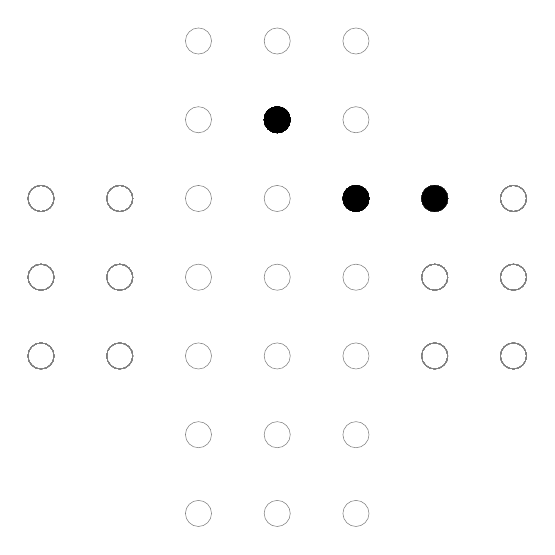
\begin{tikzpicture}
        [empty/.style={circle,draw=gray,very thin}, full/.style={circle,draw=black, fill=black ,very thin}]
        \foreach \x in {2,3,4}
          \foreach \y in {0,1, 2,3,4,5,6}
            \path node at (\x,\y) [empty] {}
                  node at (0,2) [empty] {}
                  node at (0,3) [empty] {}
                  node at (0,4) [empty] {}
                  node at (1,2) [empty] {}
                  node at (1,3) [empty] {}
                  node at (1,4) [empty] {}
                  node at (5,2) [empty] {}
                  node at (5,3) [empty] {}
                  node at (5,4) [empty] {}
                  node at (6,2) [empty] {}
                  node at (6,3) [empty] {}
                  node at (6,4) [empty] {}
                  node at (4,4) [full] {}
                  node at (5,4) [full] {}
                  node at (3,5) [full] {};
      \end{tikzpicture}
    }
    \caption{A start state}
  \end{subfigure}\hfill%
  \begin{subfigure}[t]{0.3\textwidth}
    \centering
    \resizebox{\textwidth}{!}{
      \begin{tikzpicture}
        [empty/.style={circle,draw=gray,very thin}, full/.style={circle,draw=black, fill=black ,very thin}]
        \foreach \x in {2,3,4}
          \foreach \y in {0,1, 2,3,4,5,6}
            \path node at (\x,\y) [empty] {}
                  node at (0,2) [empty] {}
                  node at (0,3) [empty] {}
                  node at (0,4) [empty] {}
                  node at (1,2) [empty] {}
                  node at (1,3) [empty] {}
                  node at (1,4) [empty] {}
                  node at (5,2) [empty] {}
                  node at (5,3) [empty] {}
                  node at (5,4) [empty] {}
                  node at (6,2) [empty] {}
                  node at (6,3) [empty] {}
                  node at (6,4) [empty] {}
                  node at (3,4) [full] {}
                  node at (3,5) [full] {};
      \end{tikzpicture}
    }
    \caption{The right most peg jumps over its left neighbour}
  \end{subfigure}\hfill%
  \begin{subfigure}[t]{0.3\textwidth}
    \centering
    \resizebox{\textwidth}{!}{
      \begin{tikzpicture}
        [empty/.style={circle,draw=gray,very thin}, full/.style={circle,draw=black, fill=black ,very thin}]
        \foreach \x in {2,3,4}
          \foreach \y in {0,1, 2,3,4,5,6}
            \path node at (\x,\y) [empty] {}
                  node at (0,2) [empty] {}
                  node at (0,3) [empty] {}
                  node at (0,4) [empty] {}
                  node at (1,2) [empty] {}
                  node at (1,3) [empty] {}
                  node at (1,4) [empty] {}
                  node at (5,2) [empty] {}
                  node at (5,3) [empty] {}
                  node at (5,4) [empty] {}
                  node at (6,2) [empty] {}
                  node at (6,3) [empty] {}
                  node at (6,4) [empty] {}
                  node at (3,3) [full] {};
      \end{tikzpicture}
    }
    \caption{The winning state}
  \end{subfigure}
  \caption{A winning set of valid moves}
\end{figure}
\pagebreak
\section*{Solution Technique}
Recursive backtracking using depth first search was chosen as the method for state space exploration. Unlike the brute force approach to finding a solution to a game, the game tree is not fully precomputed and then explored. Instead in Algorithm \ref{standard-dfs} the tree is generated by choosing a random legal move performing it and then evaluating the resulatant state. If the resulting state is not the winning state a random legal move is chosen and performed on that state. This is repeated until a state with no legal moves is reached. If that terminal state is the winning state then the sequence of moves taken to reach that state is returned. If it is not the winning state then the algorithm backtracks to the previos state and choses a different move. Thus the game tree is generated in a depth first manner as it is explored. Due to the nature of peg solitaire it is sufficient to return the first solution found as the optimal solution (see \nameref{algo-analysis})

\begin{algorithm}[H]
	\DontPrintSemicolon
  \label{standard-dfs}
	\SetKwInOut{Input}{input}
	\SetKwInOut{Output}{output}
	\SetKwData{Result}{result}
	\SetKwData{State}{state}
	\SetKwData{Initial}{initialState}
	\SetKwData{Legal}{legalMoves}
	\SetKwData{Move}{move}
	\SetKwData{Child}{childResult}
	\SetKw{Break}{break}
	\SetKw{Continue}{continue}
	\SetKwFunction{Backtrack}{backtrack}
	\SetKwProg{Fn}{Function}{}{}
	\Fn{\Backtrack}{
		\Input{An initial, possibly un-winnable, board state.} %We can't restrict ourselves to valid states, or we wouldn't be able to recurse.
		\Output{A sequence of moves to get from the initial state to the winning state, if a winning state
			cannot be reached the sequence should be empty.}
		\BlankLine
		\Initial$\leftarrow$ The initial state\;
		\Legal$\leftarrow$ A list of all the legal moves for \Initial\;
		\Result$\leftarrow$ Empty list to store moves from the initial state to the winning state\;
		\ForEach{\Move in \Legal}{
			\State$\leftarrow$ The state after playing \Move on \Initial\;
			\If{\State is a winning state}{
				\Result$\leftarrow$ \Move\;
				\Break\;
			}
			\BlankLine
			\Child$\leftarrow$ \Backtrack{\State}\;
			\BlankLine
			\If{\Child is not empty}{
				Prepend \Move to \Child\;
				\Result$\leftarrow$ \Child\;
				\Break\;
			}
		}
		\BlankLine
		\Return{\Result}\;
	}
	\caption{A standard recursive backtracking using DFS}
\end{algorithm}
But because pegs are indistinguishable, game states where pegs are in the same position are identical, regardless of the moves taken to arrive at that state. Thus exploring the state space looking for a sequence of states leading to the winning state will probably involve evaluating the same states many times. Thus a significant speed up can be achieved by saving states that are known to not lead to the winning state as shown in Algorithm \autoref{dyn-alg}. A hash set of infeasible states is kept as the game tree is explored with states inserted into this set if it is not a winning state and there are no legal moves from that set or if all of its children are already in the set.
\begin{algorithm}[H]
	\DontPrintSemicolon
  \label{dyn-alg}
	\SetKwInOut{Input}{input}
	\SetKwInOut{Output}{output}
	\SetKwData{Result}{result}
	\SetKwData{State}{state}
	\SetKwData{Initial}{initialState}
	\SetKwData{Legal}{legalMoves}
	\SetKwData{Move}{move}
	\SetKwData{Child}{childResult}
	\SetKwData{Dataset}{infeasibleSet}
	\SetKw{Break}{break}
	\SetKw{Continue}{continue}
	\SetKwFunction{Backtrack}{dynamicBacktrack}
	\SetKwProg{Fn}{Function}{}{}
	\Fn{\Backtrack}{
		\Input{An initial, possibly un-winnable, board state.}
		\Input{A set of all states that have been searched and are known to be un-winnable.}
		\Output{A sequence of moves to get from the initial state to the winning state, if a winning state
			cannot be reached the sequence should be empty.}
		\BlankLine
		\Initial$\leftarrow$ The initial state\;
		\Dataset$\leftarrow$ The set of un-winnable states\;
		\Legal$\leftarrow$ A list of all the legal moves for \Initial\;
		\Result$\leftarrow$ Empty list to store moves from the initial state to the winning state\;
		\ForEach{\Move in \Legal}{ \label{loop}
			\State$\leftarrow$ The state after playing \Move on \Initial\;
			\BlankLine
			\If{\State is in \Dataset}{
				\Continue\;
			}
			\BlankLine
			\If{\State is a winning state}{
				\Result$\leftarrow$ \Move\;
				\Break\;
			}
			\BlankLine
			\Child$\leftarrow$ \Backtrack{\State, \Dataset}\;
			\BlankLine
			\uIf{\Child is not empty}{
				Prepend \Move to \Child\;
				\Result$\leftarrow$ \Child\;
				\Break\;
			}
			\Else{
				Add \State to \Dataset\;
			}
		}
		\BlankLine
		\Return{\Result}\;
	}
	\caption{Recursive backtracking using DFS and dynamic programming methods}
\end{algorithm}

\section*{Analysis}
\subsection*{Algorithmic Analysis}\label{algo-analysis}
For any given state $S$ let $P$ be the number of pegs and $E$ be the number of empty spaces.
There are 33 spaces on a board so $E=33-P$

For any legal move a peg must jump over an orthoganal neighbour and that neighbour is then removed. Therefore for any initial state a solution must consist of exactly $P-1$ moves. If more moves were performed then there would be no pegs left and if fewer were performed the resultant board wouldn't be the final state.
The best case for a depth first algorithm is going to be if the correct move was selected and performed at each level of the tree, thus the best case for our backtracking DFS, with or without the dynamic programmng methods,  would be $O(P-1)=O(P)$

On the other hand the worst case would be when the entire game tree has to be explored to find a solution. One can estimate an upper bound on the number of legal moves that can be made in any given game state in two ways. Firstly pegs have to jump orthoganaly so each peg could jump, at most, in 4 directions. Alternatively since pegs have to jump into empty spaces, each empty space could be jumped into by at most 4 pegs. For a state that has 32 pegs and 1 empty space, e.g. the standard start state, there only 4 legal moves. Whereas in a state with 2 neighbouring pegs and 31 empty spaces there are only 2 possible moves. Therefore an upper bound on the number of moves could be the minimum$\{4P,4E\}$ but $4P<4(33-P)$ $\forall P\leq16$ giving an upper bound of $4\times16=64=2^6$ on the number of moves that can be made in any state.

As discussed above the number of moves to find a solution is $P-1$ but for some invalid paths the moves may lead to an invalid state that while $P>1$, no legal moves can be performed due to the relative positions of the remaining pegs. Thus $P-1$ is an upper bound on the depth with which any branch must explored, i.e. the maximum height of the game tree is $P-1$.

If we consider the root node to be at depth $0$ of the tree, at depth 1 there are at most $2^6$ states, at depth 2 there are $(2^6)^2$ states. Following this pattern, at the maximum depth of $P-1$ there are $(2^6)^{P-1}$ terminal states. Therefore the total number of states in the game tree is $1+(2^6)+(2^6)^2+(2^6)^3+...+(2^6)^{P-1}=\sum_{i=0}^{i=P-1} (2^6)^i=\frac{(2^6)^P-1}{(2^6)-1}$
Therefore the worst case would be $O(2^{P})$ which is equivalent to $O(2^{N})$ where $N$ is the number of moves in the solution.
\subsection*{Empirical Analysis}
\graphicspath{ {TestData/} }
\begin{figure}[h]
  \includegraphics[width=\linewidth]{time_vs_nodes}
  \caption{Graph comparing running time with the number of elements searched}
  \label{tvn_graph}
\end{figure}
\autoref{tvn_graph} shows that the running time can be fit to the line $2133.73x^{1.083}$ with an $R^2$ value of $0.81$ meaning the algorithm is of $O(n^{0.81}) \approx O(n)$ complexity in the number of elements of the tree searched.

\begin{figure}[h]
	\includegraphics[width=\linewidth]{time_vs_length}
	\caption{Graph comparing running time with the length of the solution found}
	\label{tvl_graph}
\end{figure}

\autoref{tvl_graph} shows that the running time can be fit to the line $2000 e^{0.6x}$ meaning the algorithm is of $O(e^n)$ complexity in the length of the solution.

\end{document}
